\section{Frontend}

The evaluation of the Elephant browser and the NetInfService applications tries to answer the following two core questions:

\begin{enumerate}
\item How much uplink bandwidth is saved?
\item How much of content is used multiple times throughout web pages?
\item How much of linked resources are dynamically generated?
\item How much time does it take to retrieve web page?
\end{enumerate}

\subsection{Test Setup}

The first test setup consists of a set of web pages from which each of four Android phones will automatically retrieve 15 in a random order. Using the logging functionality of the applications, information about how (Internet, Bluetooth, NRS or Database) resources are retrieved, how many bytes each resource consists of and how long it take to retrieve are acquired. The results are meant to give an idea of the answer to questions 1 and 2.

The web page sets are of sizes 15, 20, 25, 30 and 35. They are derived from the service Alexa \cite{alexa}, which is renowned for its web metrics. This service keeps track of the most visited web sites by country, and the top sites were used to create the sets.

For the backend the setup for the tests consist of a Name Resolution Service that is reset between each test.

The second test setup consisted of first retrieving all web pages from the set of 30 using one phone, and then repeat. The results are meant to give an idea of the answer to question 3. The test is repeated two times. 

\subsection{Hardware}

Tests are run on three Samsung Galaxy Nexus phones and one HTC One X phone using Android OS 4.1.1 Jellybean that were provided by Ericsson.

For the backend the Name Resolution Service was run on a Intel Core 2 Quad CPU Q9400 @ 2.66GHz × 4 with 4 gigabytes of memory using Ubuntu 12.04 LTS.

\subsection{Limitations}

The backend Name Resolution Service supports two types of databases to use for storing published NDOs. The first uses Erlang lists stored in main memory, the other uses a Riak database. The list database was chosen for this test as it is more well tested and easier to work with.

This however means that the test is limited to using the free main memory of the system. A preliminary test using a set of 50 web pages caused the system to run out of memory, resulting in a crash. Therefore, the size of the sets are limited to a maximum of 35 web pages.

\subsubsection{Results}

% Plot of usage

% Table comparing time of access to each resource

% Table (or plot) of re-usage after period

The results of test one can be seen in Figure \ref{fig:frontendtest2}. Each bar represents a specific set size and the colors show how much of the data was transferred with each technology.

\begin{figure}
	\centering
		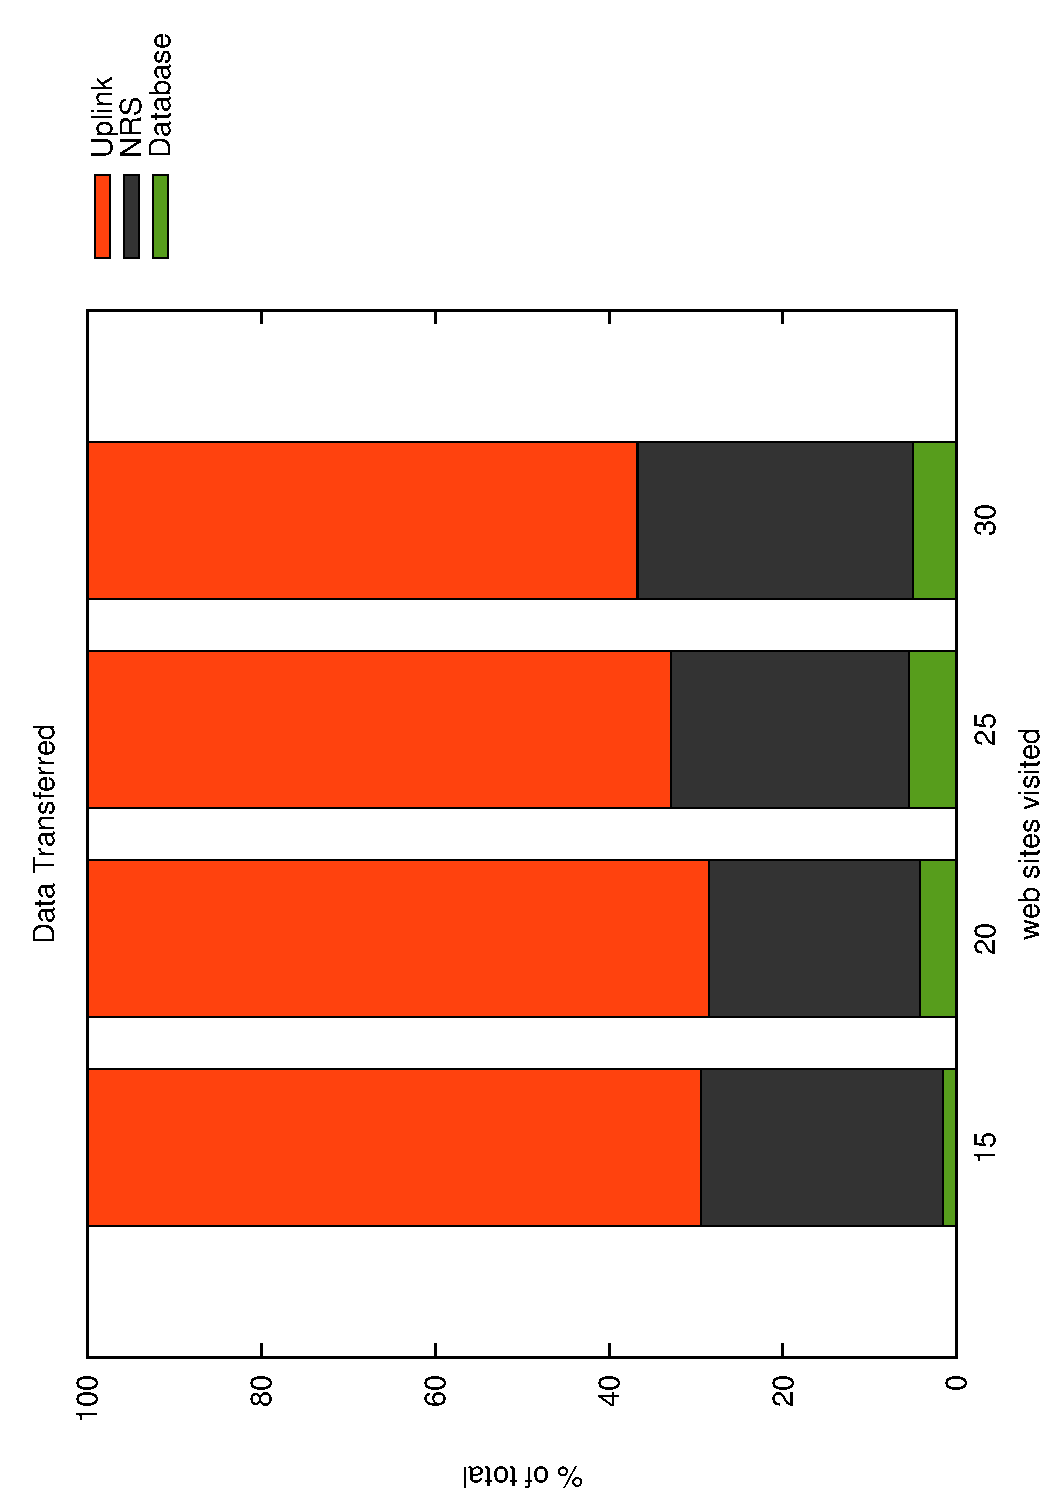
\includegraphics[width=0.75\textwidth, angle=-90]{./img/plots.pdf}
    	\caption{Results of Test 1}
	\label{fig:frontendtest1}
\end{figure}

The results of test two can be seen in Figure \ref{fig:frontendtest2}. The two leftmost bars represent the first repetition of the test and the two right most the second repetition.

\begin{figure}
	\centering
		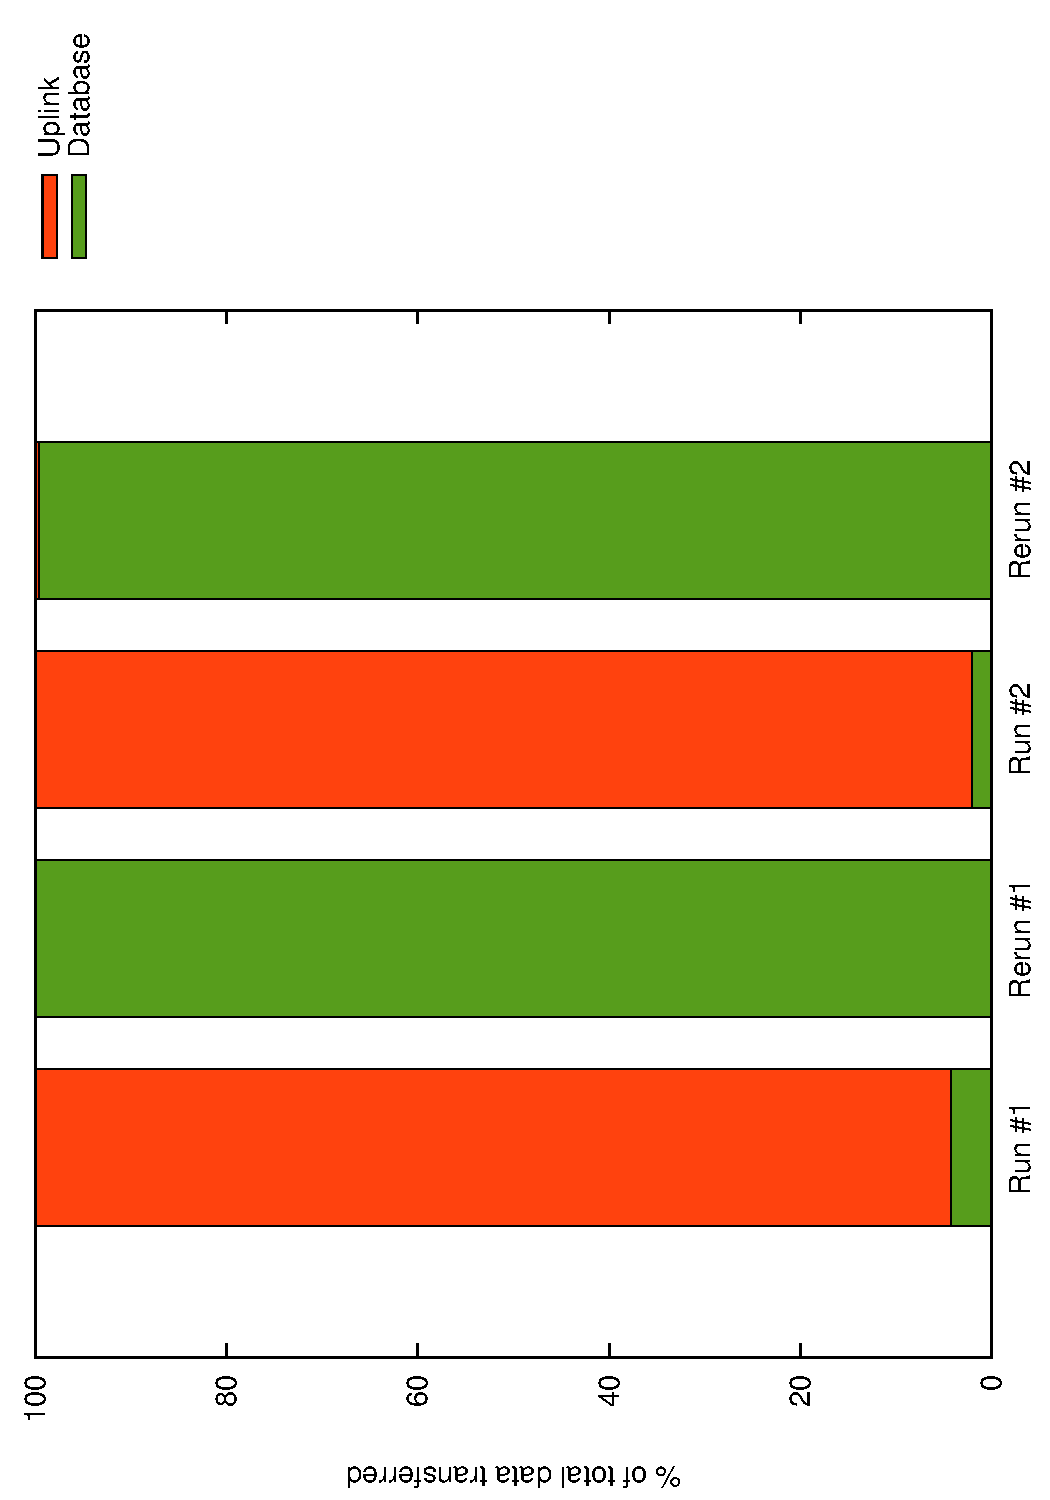
\includegraphics[width=0.75\textwidth, angle=-90]{./img/rerun.pdf}
    	\caption{Results of Test 2}
	\label{fig:frontendtest2}
\end{figure}

\subsubsection{Discussion}

From Figure \ref{fig:frontendtest1}, we can see that even without precaching and even when the phones are not downloading exactly the same web pages, approximately 30\% of the data can be retrieved without using the Internet. With precaching of popular web pages this percentage could possibly increase even further.

One could expect the amount of data retrieved from the Internet to drastically increase as the number of web pages in the set increase since fewer and fewer pages will be retrieved by all phones. This does however not seem to be the case, at least for these set sizes, as can be seen in Figure \ref{fig:frontendtest1}. One possible explanation is that when there are fewer web pages in the set multiple the chance of multiple phones retrieving the same web page at the same time increases. If one phone had a jump start on another phone to start retrieving a certain web page, the second phone shortly caught up with the first phone. The two phones then try to retrieve the same resource at the same time which will not be in the cache and both will use the Internet.

In Figure \ref{fig:frontendtest1} it can also be seen that a few percent of resources are retrieved from the database. This is because these resources are linked to several times throughout the web pages. Since the resource is cached in the database the first time, additional requests can use the database.

From Figure \ref{fig:frontendtest2} we can see that when accessing a web page a second time a small part still has to be retrieved using the Internet. An example of when this can happen is when a web page links to a resource using JavaScript to add a timestamp to the resource's URL. The dynamic nature of this content means that it will not be in any cache when requested. This means there will be a certain amount of resource that will have to be retrieved from the Internet.

From Table TODO REF it can be seen that the retrieval of web pages is very slow. So slow that using this application in a real life situation probably only makes sense if there is no connection at all otherwise. The main culprit behind the long retrieval times seems to be the search. Since a search is done for every web resource the time quickly adds up. To improve the retrieval times of web pages the search needs to be optimized.

One thing that is not immediately visible but that effects the test result is the fact that NetInfService randomly pauses in the background. If this happens it results in all publishes, gets and searches failing which in turn results in everything being retrieved from the Internet. It is suspected that this is caused by how the Android OS handles applications in the background.